\documentclass[12pt,a4paper]{article}
\usepackage[a4paper,left=2cm,right=2cm,top=2cm,bottom=4cm]{geometry}
\usepackage[utf8]{inputenc}
\usepackage[T1]{fontenc}
\usepackage{amsmath}
\usepackage[ngerman]{babel}
\usepackage{amssymb}
\usepackage{float}
\usepackage{graphicx}
\usepackage{titling}

\usepackage{xcolor}
\usepackage{titlesec}



\definecolor{xsens}{RGB}{0,115,188}
\usepackage{sectsty}
%\chapterfont{\color{xsens}}  % sets colour of chapters
%\sectionfont{\color{xsens}}  % sets colour of sections
%\chapterfont{\color{xsens}}


\author{Mirco Huber}
\newcommand{\subtitle}{Ausmessung Prototypen}
\title{NORD-LOCK SUPERBOLT}


%%%%%%%%%%%%%%%%%% HEADER AND FOOTER
\usepackage{fancyhdr}
\setlength\headheight{40pt}
\renewcommand{\headrulewidth}{0pt}

\lhead{\thetitle}
\rhead{
\includegraphics[height=4em]{Logos/X-SENSORS-Logo_Slogan_EN_Transparent.png}}
\rfoot{\thepage}
\cfoot{}

\fancypagestyle{plain}{%
	\setlength\headheight{40pt}
	\renewcommand{\headrulewidth}{0pt}
	\lhead{\thetitle}
	\rhead{
\includegraphics[height=4em]{Logos/X-SENSORS-Logo_Slogan_EN_Transparent.png}}
	\rfoot{\thepage}
	\cfoot{}
	
}

\fancypagestyle{empty}{%
	\fancyhf{}
}

\usepackage{subfiles}

\titleformat{\chapter}[display]
{\normalfont\huge\bfseries}{}{0pt}{\thechapter.\ }

\usepackage{nicefrac}
\usepackage{tocloft}


\pagestyle{fancy}
\begin{document}
	\thispagestyle{empty}
	\begin{titlepage}
		\begin{figure}[H]
			\centering
			
\includegraphics[width=.5\linewidth]{Logos/X-SENSORS-Logo_Slogan_EN_Transparent.png}
		\end{figure}
		\vspace*{3cm}
		\begin{center}
			\Huge {\thetitle} \\\vspace*{.5cm}
			\small {\subtitle}
		\end{center}
		\vspace{12cm}
		\hspace{.6\linewidth} 
		\begin{tabular}{l}	
			\small{\theauthor} \\[.5pt]  
			\small{X-Sensors AG} \\ 
			\small{Landenbergerstrasse 13} \\
			\small{CH-8253 Diessenhofen} \\ [.5cm] 	
			\today
		\end{tabular}
	\end{titlepage}

	\newpage
	\setcounter{page}{1}
	\pagenumbering{arabic} % A-Z Seiten (werden ausgeblendet), geht nur um PDF
	\pagestyle{fancy}
	
	
	
	%%%%%%%%%%%%%%%%%%%%%%%%%%%
	\section{Messkurve DUT1}
	\begin{figure}[H]
		\centering
		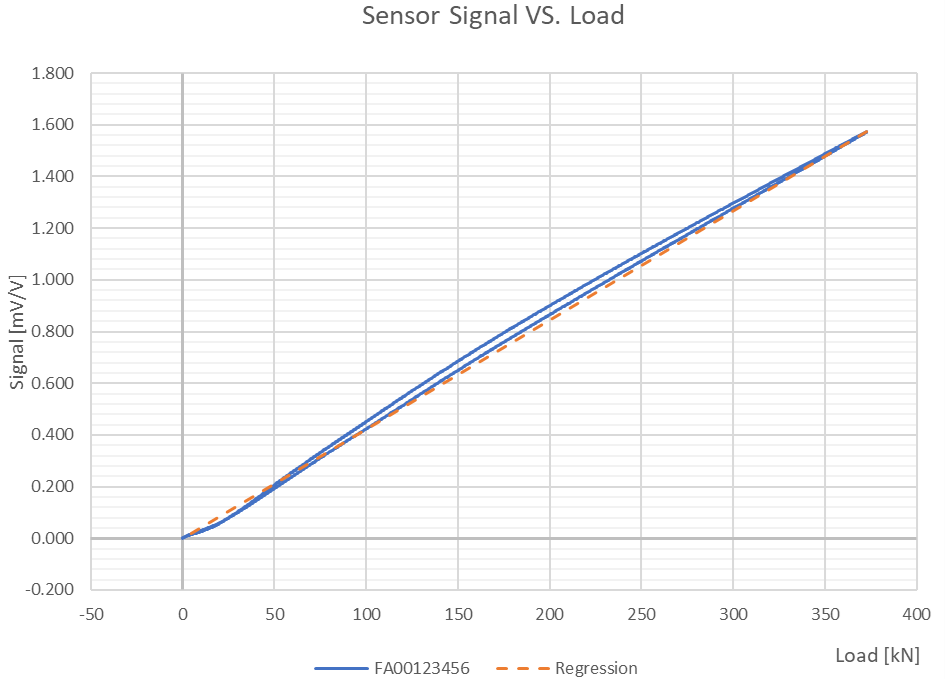
\includegraphics[width=.8\linewidth]{img/screenshot001}
%		\caption{Messkurve DUT1}
		\label{fig:screenshot001}
	\end{figure}
	\begin{figure}[H]
		\centering
		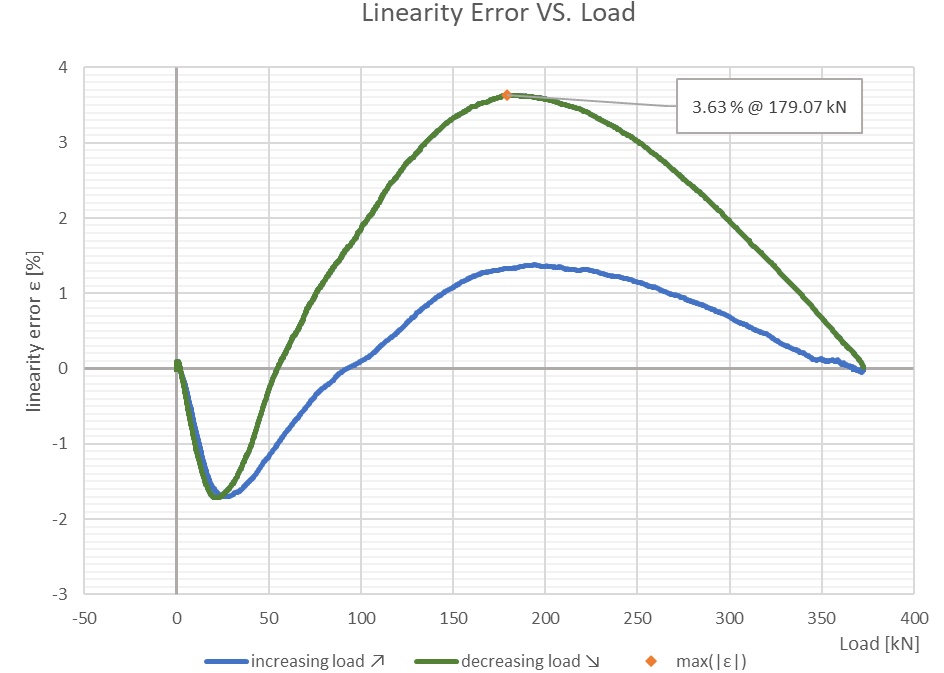
\includegraphics[width=.8\linewidth]{img/screenshot002}
%		\caption{Linearitätsfehler / Hysterese DUT1}
		\label{fig:screenshot002}
	\end{figure}
	\section{Messkurve DUT2}
\begin{figure}[H]
	\centering
	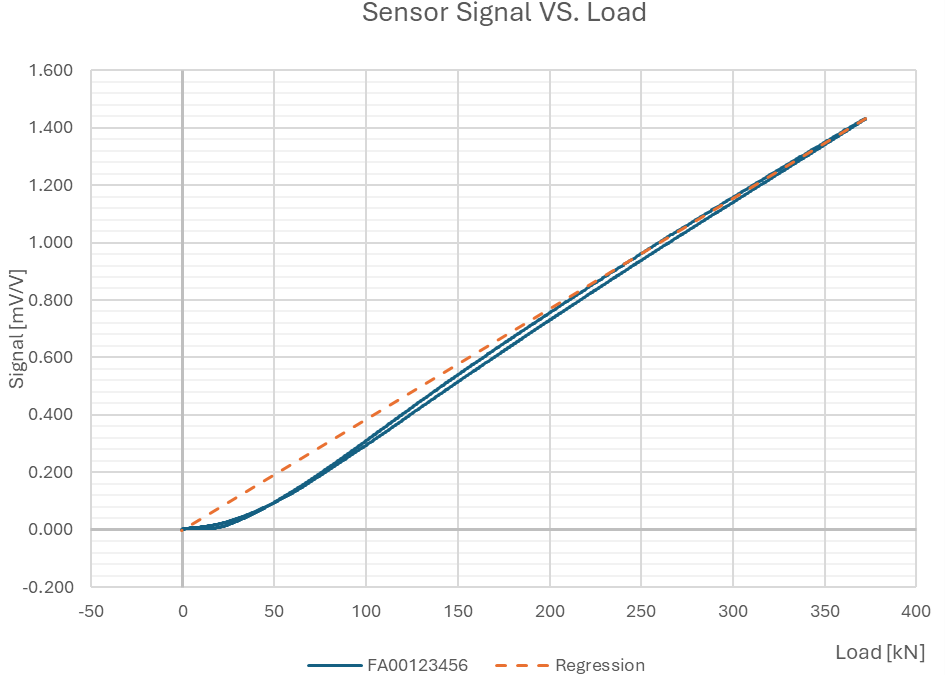
\includegraphics[width=.8\linewidth]{img/screenshot003}
%	\caption{Messkurve DUT2}
	\label{fig:screenshot003}
\end{figure}
\begin{figure}[H]
	\centering
	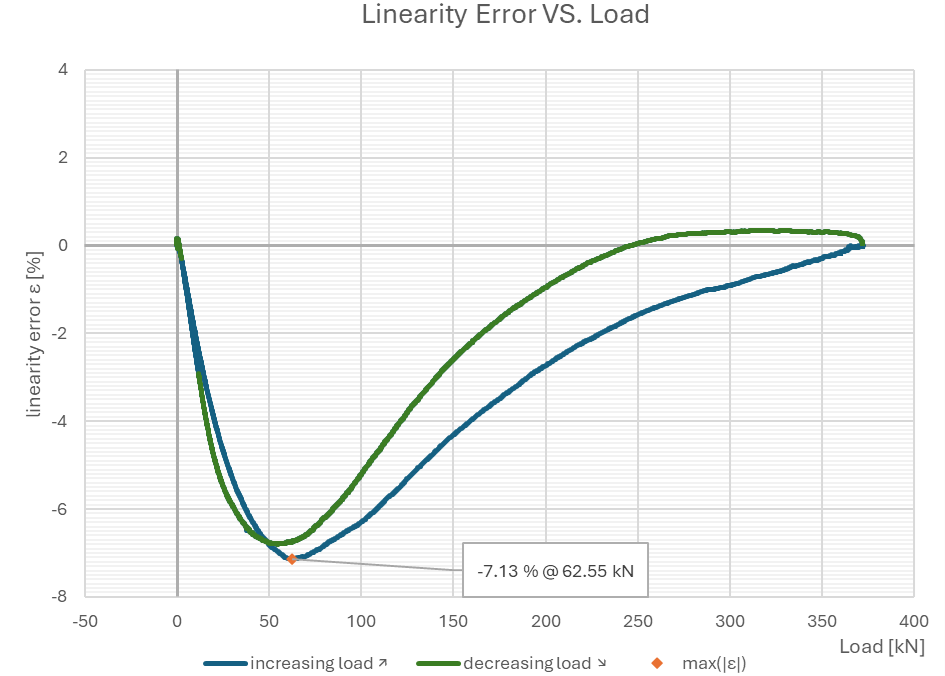
\includegraphics[width=.8\linewidth]{img/screenshot004}
%	\caption{Linearitätsfehler / Hysterese DUT2}
	\label{fig:screenshot004}
\end{figure}
	\section{Messkurve DUT3}
\begin{figure}[H]
	\centering
	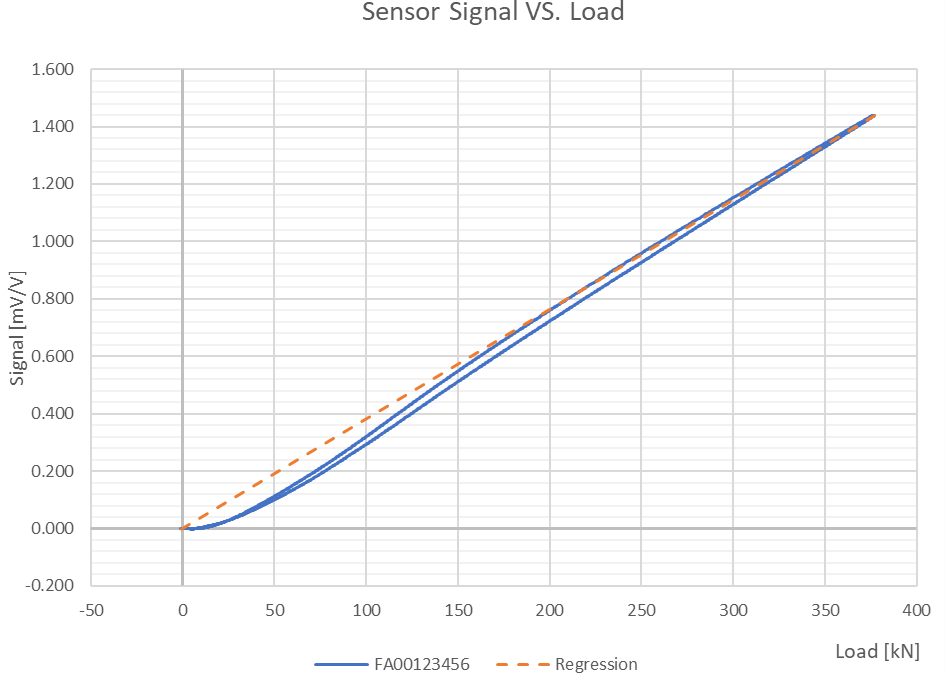
\includegraphics[width=.8\linewidth]{img/screenshot005}
%	\caption{Messkurve DUT3}
	\label{fig:screenshot005}
\end{figure}
\begin{figure}[H]
	\centering
	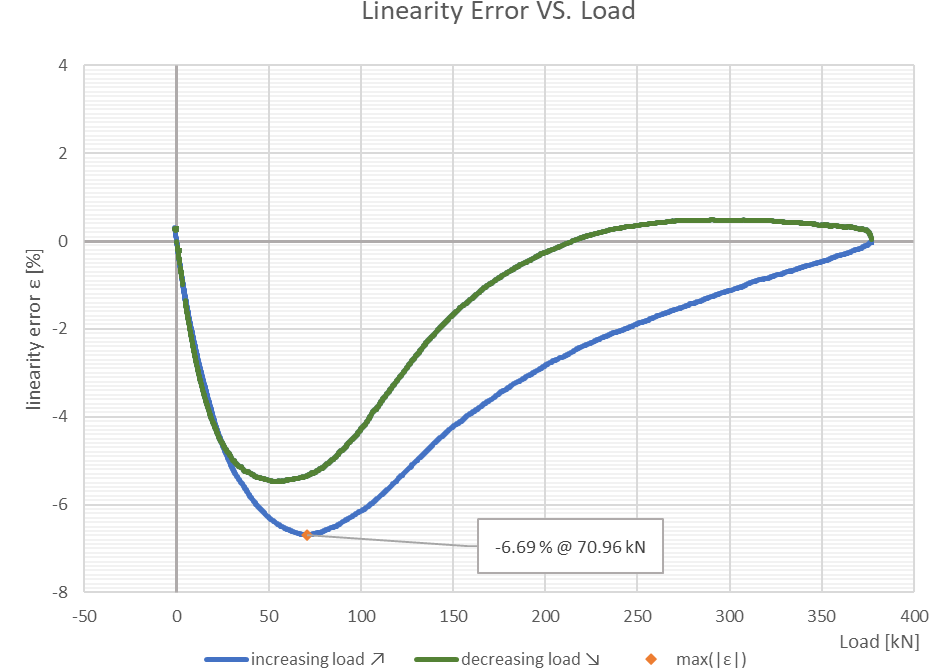
\includegraphics[width=.8\linewidth]{img/screenshot006}
%	\caption{Linearitätsfehler / Hysterese DUT3}
	\label{fig:screenshot006}
\end{figure}
	\section{Messkurve DUT4}
\begin{figure}[H]
	\centering
	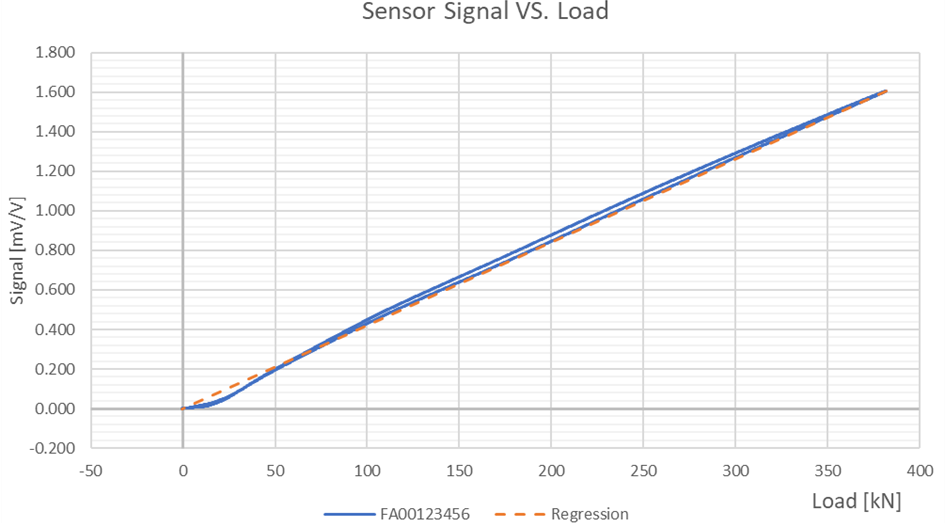
\includegraphics[width=.8\linewidth]{img/screenshot007}
%	\caption{Messkurve DUT4}
	\label{fig:screenshot007}
\end{figure}
\begin{figure}[H]
	\centering
	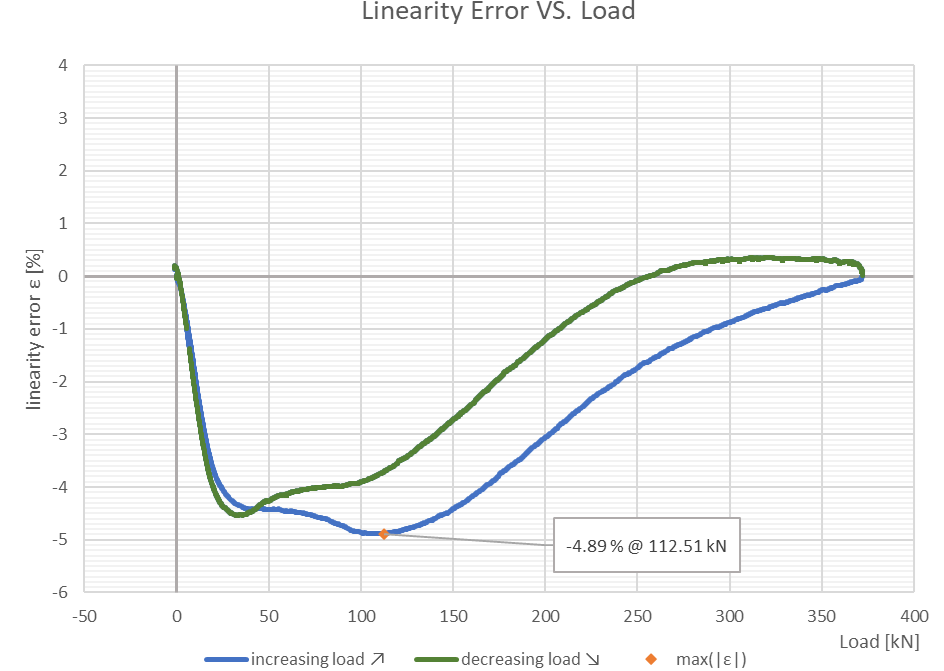
\includegraphics[width=.8\linewidth]{img/screenshot008}
%	\caption{Linearitätsfehler / Hysterese DUT4}
	\label{fig:screenshot008}
\end{figure}
	\section{Messkurve DUT4 90$^\circ$ gedreht }
\begin{figure}[H]
	\centering
	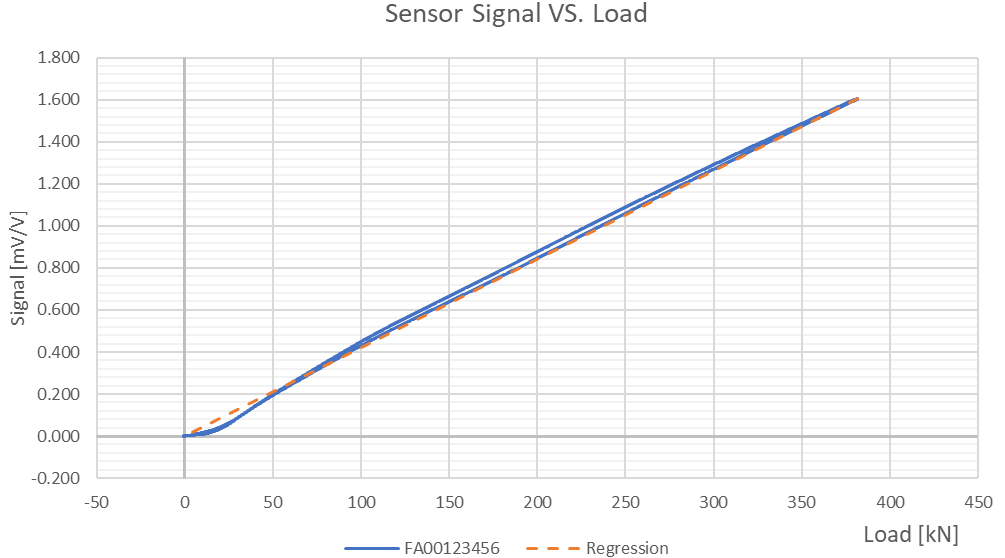
\includegraphics[width=.8\linewidth]{img/screenshot009}
%	\caption{Messkurve DUT4 90 $^\circ$ gedreht}
	\label{fig:screenshot009}
\end{figure}
\begin{figure}[H]
	\centering
	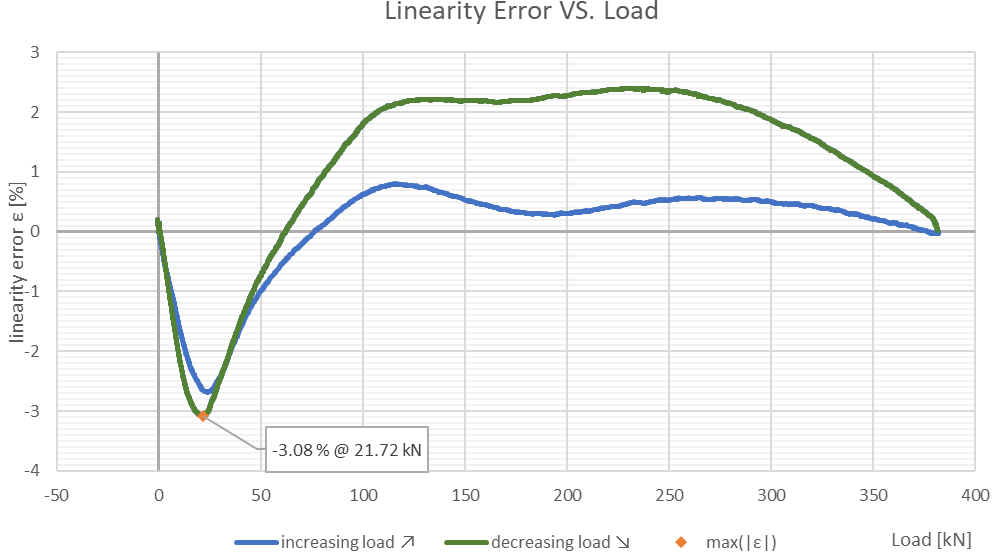
\includegraphics[width=.8\linewidth]{img/screenshot010}
	%\caption{Linearitätsfehler / Hysterese DUT4 90 $^\circ$ gedreht}
	\label{fig:screenshot010}
\end{figure}
	

\end{document}